\chapter{Analyses} % Main chapter title

\label{Chapter:Analyses}

As presented in Fig. \ref{fig:sustainableCityFramework}, the indicators for measuring a sustainable city are categorised into economic, social and environmental. This section of the paper discusses the nexus between urban agriculture and sustainable cities with reference to the indicator-sets under each of the themes.

\section{Urban agriculture and economic sustainability of cities}

\subsection{Full-time employment}

Urban agriculture provides employment, and has thus become a major means of livelihood, for people in many cities particularly in the global south (Darkey et al., 2014; Zezza \& Tasciotti, 2010). An estimated 2100 farm labourers in Morogoro and 6400 in Mbeya, Tanzania are engaged in urban agriculture as either attendants or fodder collectors (International Labour Organization, 2013). Similarly, approximately 120,000 low-income households (including farmers, garland makers and garland sellers) in Manila, Philippines depend on jasmine production for their livelihoods (IPC, 2007). Many examples of urban agriculture's role in employment creation abound in the conventional literature (see: Amponsah et al., 2015a; Carr, Potter, \& Nortcliff, 2011; Sinclair, 2010; Tiongco, Narrod, \& Bidwell, 2010). The general observation is that urban agriculture's role in employment creation is widespread in the global south as depicted in Table \ref{tbl:peopleEngagedInUA}.

\begin{table}[th]
\caption{Number of people engaged in urban agriculture in the global south. Source: FAO (2007).}
\begin{center}
\begin{tabular}{ p{0.20\textwidth} p{0.25\textwidth} p{0.45\textwidth} } 
\hline
Region & Number (million) & Principal live-hood \\
\hline
Sub-Saharan Africa & 11 & Commercial vegetable growing or dairy farming \\
Northern Africa and the Middle East region & 6 & Horticultural and livestock products (fruit, vegetables and poultry) \\
South Asia & 11 & Perishable high-value commodities such as milk and fresh vegetables \\
East and South-East Asia & 7 & Perishable high-value commodities such as milk and fresh vegetables \\
\hline
\label{tbl:peopleEngagedInUA}
\end{tabular}
\end{center}
\end{table}

Not only is urban agriculture a source of employment to farmers but also to stakeholders along the value chain (Fig. 2). Community and farmers' markets and door-to-door delivery of food baskets in Argentina, Brazil and Uruguay are examples of jobs created in the commercial sector by urban agriculture (International Labour Organization, 2013). Similarly, majority of vegetable farmers in urban and peri-urban Ghana deliver their produce to wholesalers, who are predominately women, at the farm-gate (Abaidoo et al., 2009; Amoah, Drechsel, Henseler, \& Abaidoo, 2007; Amponsah et al., 2016). These wholesalers in turn sell the produce to retailers, food vendors and households as depicted in Fig. 2. The farm produce is conveyed from the farm-gate to the open markets by transport operators.

The discussion so far suggests that urban agriculture makes a profound contribution to the employment of the labour force in the global south. The situation differs from the cities in the global north because the narrative in the conventional literature suggests that the motivation for urbanites and city authorities to promote agriculture in these cities lies in its ecological functions as well as its support for leisure and recreation (Pearson et al., 2010). The implication is that the role of urban agriculture in employment creation in the global north may not be as profound as it is in the global south. This is because, urban agriculture in the global north is not economically-centred but rather centred on its environmental functions. Nonetheless, recent studies give indications that the functions of urban agriculture in the global north is gradually shifting from leisure and recreation to more of urban sustainability and economic resilience (Lovell, 2010; McClintock, 2010). The increasing focus on economic resilience means that the contribution of urban agriculture in the global south and north appears to be converging even though there are variations across cities. Nevertheless, if the agricultural lands had been used for non-agricultural purposes, the employment effects may have been more profound. For instance, industrial and commercial activities on these parcels of land may have made more profound contributions to employment creation.

\subsection{Employment for women}

According to Prain and Lee-Smith (2010), two out of every three urban farmers in Yaounde, Nakuri, Maputo, Nairobi and Kampala are women. Generally, these women farmers engage in subsistence farming with the objective of meeting the family demand for fresh, nutritious and chemical-free food (Gamhewage, Sivashankar, Mahaliyanaarachchi, Wijeratne, & Hettiarachchi, 2015). The rest of the urban women farmers sell the excess produce for income. However, agriculture could be a burden to these women due to the numerous roles they perform at the household level. The argument does not pertain to agriculture but also applies to almost all the economic activities the women are engaged in. The implication is that without addressing the issues that foster gender inequality, women's engagement in agriculture in the cities could be a burden (Veenhuizen, 2006). There must therefore be a conscious effort by policy makers and social advocates to help minimise the pressure on women emanating from the combination of household chores and economic activities such their involvement in urban agriculture.

Generally, commercial urban agriculture is dominated by men as depicted in Table 2. In contrast, women are dominant at the market and food vending stages of the supply chain (Drechsel & Keraita, 2014). It can therefore be deduced that commercial agriculture in the cities in the global south is gendered and thus makes a profound contribution to


%\begin{figure}[th]
%\centering
%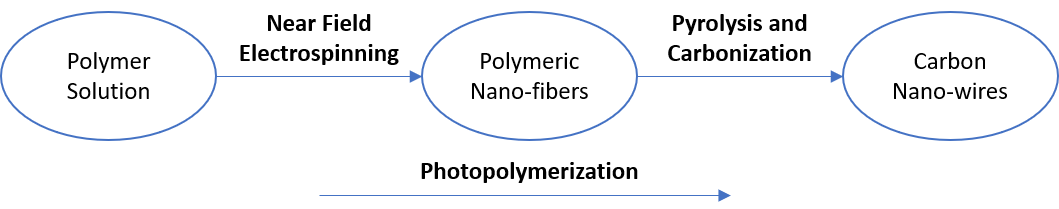
\includegraphics[width=0.95\textwidth]{./Figures/FabricationProcess.png}
%\decoRule
%\caption[Carbon Nano-wires Fabrication Process]{Fabrication process of carbon nano-wires to achieve through the proposed dissertation.}
%\label{fig:fabricationFlowChart}
%\end{figure}

%\begin{equation}
%\left(\tau _t^e-\frac{\tau _n^e \text{dr}}{\text{dz}}\right) 2 \pi  r+\frac{d \left(\pi  r^2
%   \left(\tau _{\text{zz}}-p\right)\right)}{\text{dz}}+\frac{\gamma  \text{dr} 2 \pi  r}{r
%   \text{dz}}+\rho  g \pi  r^2=\frac{d \left(\rho  \pi  r^2 v^2\right)}{\text{dz}}
%\label{eq:linearMomentum}
%\end{equation}